%!TEX root = ../main.tex
% !TeX spellcheck = en_GB 


\chapter{Implementation}
\label{chap_impl}
The objective of this thesis has been to implement and evaluate a  collision avoidance  algorithm for USVs. Several related approaches were analysed before the fuzzy logic approach presented by \textcite{perera2012intelligent}, was chosen.
The solution presented in the original paper is implemented in MATLAB, while the solution presented here is implemented in Python. Python was chosen due to the writer's previous knowledge of the language as well as the availability of fuzzy logic python libraries. The library used in this implementation is called SciKit-Fuzzy \cite{josh_warner_2017_1002946}.

\section{The fuzzy inference system}
SciKit-Fuzzy provides a simple application programming interface to set up a FIS. This section will describe the process setting up a simple FIS that calculates salary based on age and the number of previous jobs, instead of the complicated navigation model. Fuzzy sets for age are set up in the same way as in \ref{sec:fuzzy_sets}, but with age ranges more appropriate for the example. The sets are therefore young = 18 - 35 years, middle-aged = 30 - 50 years, and old 45-65 years.  Additionally, job and salary sets are introduced. Line 4-6 in listing \ref{listing:fis} initializes the universes for the different fuzzy sets. These are 18-100 for age and 0-10 for jobs, both with a step of 1. Age and jobs act as antecedents in the FIS and the initialization call is therefore to  \texttt{ctrl.Antecedent} Salary goes from 1500-10000 with steps of 500 and acts as consequent and is therefore initialized with  \textit{ctrl.Consequent}. The numbers used are made up for the sake of the example.

Next, the membership functions are initialized in lines 7-15. The age sets are defined  on lines 7-9 as described above.
Three different job sets are defined: \textit{few} (<3),  \textit{medium} (2-6), and \textit{many} (>5). The salary sets are \textit{low} (1500 - 2500),  \textit{medium} (2000-7000), and \textit{high} (<6000). All sets are initialized using \texttt{fuzz.trimf} which produces a triangular membership function. The resulting FMFs are visualized in figure \ref{fig:fmf_ex3}
\begin{figure}[H]
    \centering
    \begin{tabular}{c}

        \subfloat[Age antecedent]{
            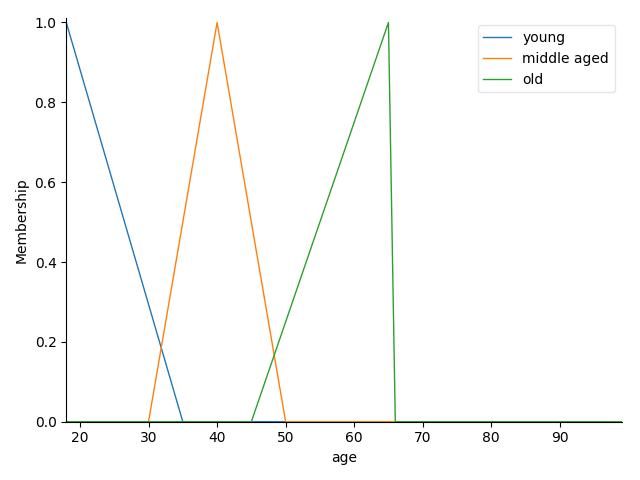
\includegraphics[width=\textwidth,height=0.30\textheight,keepaspectratio]{Figures/age_ex}
            \label{fig:age_ex}
        } \\
        \subfloat[Jobs antecedent]{
            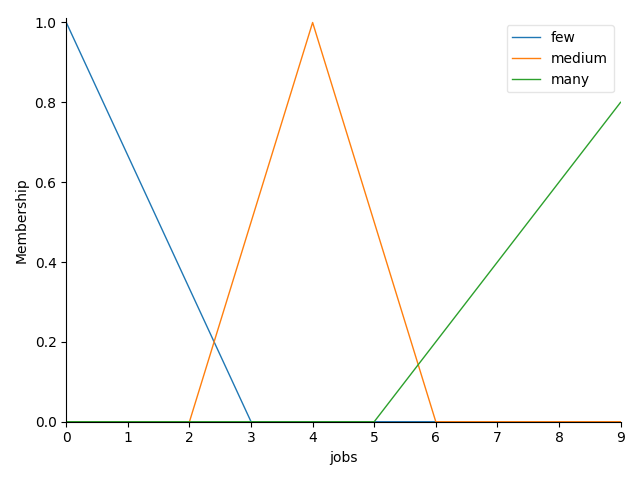
\includegraphics[width=\linewidth,height=0.30\textheight,keepaspectratio]{Figures/jobs_ex}
            \label{fig:jobs_ex}
        } \\
        \subfloat[Salary consequent]{
            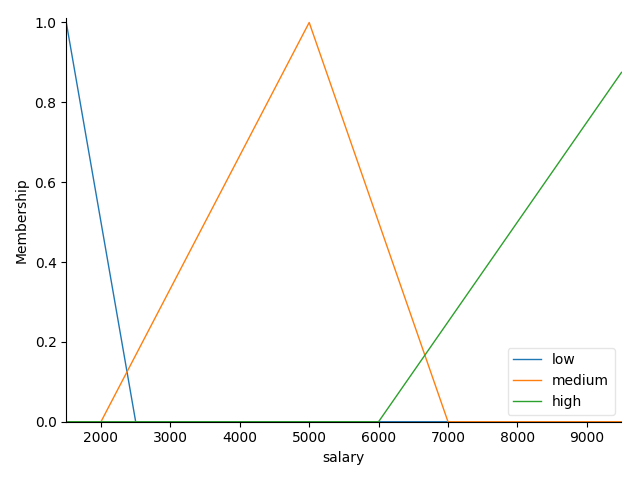
\includegraphics[width=\linewidth,height=0.30\textheight,keepaspectratio]{Figures/salary_ex}
            \label{fig:salary_ex}
        }
    \end{tabular}

    \caption{FMSs used in example FIS}
    \label{fig:fmf_ex3}
\end{figure}

Next, the following rules are defined, on lines 16 -21, to connect the antecedents with the consequents:

\begin{enumerate}[label=\textbf{Rule \arabic*},ref=Rule \arabic*]
    \item IF young  OR few jobs THEN salary is low
    \item IF middle-aged  AND few jobs THEN salary is low
    \item IF middle-aged  OR medium amount of  jobs THEN salary is medium
    \item IF middle-aged  AND many jobs THEN salary is high
    \item IF old  OR many jobs THEN salary is high
\end{enumerate}

Finally, the rules are passed to the Control System on line 25  and  \\ \texttt{ctrl.ControlSystemSimulation} is called to complete the FIS initialization.
The system is now ready to take input and calculate  an output based on the rule set specified. An example using age = 35 and jobs = 1 is input on lines 25-28 and the output printed on lines 30-32. The example outputs a salary of 4157.





\begin{listing}[H]
    \inputminted[linenos, breaklines=true,fontsize=\scriptsize, numberblanklines=false]{python}{../src/example.py}
    \caption{FIS initialization}
    \label{listing:fis}
\end{listing}

\section{Architecture}
This section  presents the high-level structure of the implementation with help of the class diagram seen in figure \ref{fig:class_diagram}. Each class and their interactions will be briefly presented.
\begin{figure}[H]
    \centering
    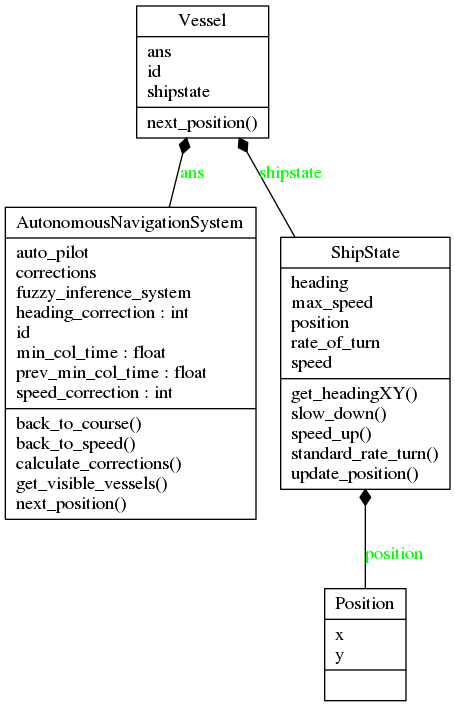
\includegraphics[width=\textwidth,height=0.75\textheight,keepaspectratio]{../src/classes_Pyreverse}
    \caption{Class diagram}
    \label{fig:class_diagram}
\end{figure}
\subsection{Classes}
Each simulation scenario consists of at least one vessel. The vessels are represented by the \textit{Vessel} class. The current state of the vessel is represented by the \textit{ShipState} class which also contains the \textit{Position} class. Furthermore, each vessel needs a navigation system, which is represented by the \textit{AutonomousNavigationSystem} class. The classes are  more thoroughly presented in the following subsections.
\subsubsection{Vessel}
\textit{Vessel} is the main class and the class with which the simulation script interacts.
It contains, apart from the previously mentioned \textit{AutonomousNavigationSystem} and \textit{ShipState} an id and a method to calculate its position in the next time frame.
A new vessel object is created with the following call:
\begin{minted}{python}
Vessel(id, heading, position_x, position_y, speed, max_speed, 
    rate_of_turn, fuzzy_inference_system, auto_pilot)
\end{minted}
This constructor call specifies the ID for the vessel as well as its initial position, speed and heading. Furthermore, it defines the vessels maximum speed and rate of turn. The two final parameters specify the fuzzy inference system to use and whether the vessel shall use the navigation system. Setting the final boolean to false creates a rogue vessel that will just keep its initial speed and heading, thereby not complying with the COLREG rules. The \textit{Vessel} class has only one method, which calculates the vessels position in the next time frame after applying possible corrections to heading and speed.
\subsubsection{Position}
The position class simply holds the vessels current coordinates in the Cartesian coordinate system used.
\subsubsection{ShipState}
ShipState holds information about the state of the vessel in the current time frame. This includes the vessels current position, heading and speed. The simulation does not distinguish between course and heading since no drift is simulated.
Furthermore, limits such as maximum allowed speed and standard rate of turn are specified in this class. Finally, the class holds methods to change the ships heading by the specified standard rate of turn or speed by 0.2 kt for acceleration and 0.7 for deceleration, until the next time frame.


\subsubsection{AutonomousNavigationSystem}
\label{sec:ANS}
The AutonomousNavigationSystem class from now on referred to as ANS is what separates an autonomous vessel from an ordinary vessel. The ANS combines the information from the ShipState class with situational awareness information provided by a separate Situational Awareness (SA) module, in order to calculate needed corrections to speed and course.

The SA is in this simulation case represented by a service that holds all the information regarding the current scenario. A real system would have a SA module that reads and processes information from different sensors, such as LiDAR and  cameras, on board the vessel. Information needed about a target vessel is its heading, speed, and position. These are used to calculate the four different inputs to the FIS system. Listing \ref{listing:rel_bear_calc} shows the method used to calculate the relative bearing passed into the FIS system. The compass bearing is first calculated from the two provided coordinate pairs after which the result is converted into a relative bearing. The relative course is then calculated as the target vessels heading - the own vessels heading, as shown in listing \ref{listing:rel_course_calc}. Distance can be obtained by using the Pythagorean theorem on the differences between the vessels in the X and Y axis. Finally, speed ratio is defined as $\frac{\text{Speed of the target vessel}}{\text{Speed of the main vessel}}$.
\begin{listing}

    \begin{minted}[linenos, breaklines=true,fontsize=\scriptsize, numberblanklines=false]{python}
rel_course = observed_vessel.shipstate.heading - shipstate.heading
if rel_course < 0:
    rel_course = 360 + rel_course
    \end{minted}
    \caption{Relative course calculation}
    \label{listing:rel_course_calc}
\end{listing}

These inputs are passed into the FIS system, for each target vessels, and the recommended corrections presented by FIS are stored in an array. The expected time until the collision for each target vessel is also calculated. Knowing the distance between the vessels, their relative velocity is needed to calculate the time. Equation \ref{eq:rel_vel_calc} shows the relative velocity calculation, based on the law of Cosines. \textit{V} stands for velocity, $\theta$ for heading, the subscript \textit{m} for own vessel and \textit{t} for target vessel.

\begin{equation}
    V_r=\sqrt{V_m^2 + V_t^2-2  V_mV_tcos(\theta_m-\theta_t)}
    \label{eq:rel_vel_calc}
\end{equation}

The previous calculations result in speed and course correction suggestions, as well as an expected time until collision, for each target vessel. However, these recommendations might contradict each other and a way to prioritize the corrections in order of urgency is therefore needed. This is solved in a simple manner by calculating the weighted arithmetic mean of the corrections using the expected time until collision as weight. The resulting correction is then stored in ShipState as target heading.

Finally, the heading and speed of the vessel are updated in the following manner. The vessels are steered towards the proposed heading change by a maximum of the vessels defined maximum rate of turn. The speed is similarly changed towards the proposed speed by a maximum of one knot. No proposed correction by the FIS means that the vessel is currently not in a scenario that satisfies a rule in the rule set. However, a previous correction suggestion might still not be completed due to the vessels limited rate of turn, acceleration or deceleration.  The vessel will, therefore, continue to change its current heading and speed towards the saved target until current and target are the same. The target is then gradually changed towards the original until they are the same. The vessel should ultimately steer back to its original track instead of course. However, this is out of the scope for this thesis. The process is visualized in figure \ref{fig:flow_chart}.
\begin{figure}[H]
    \centering
    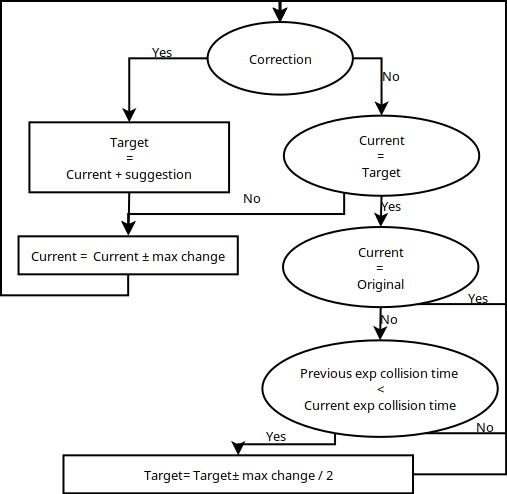
\includegraphics[width=\textwidth,height=0.75\textheight,keepaspectratio]{Figures/flow.png}
    \caption{Flow chart explaining application of heading and speed corrections}
    \label{fig:flow_chart}
\end{figure}

\section{Simulation}
The goal of the implementation is to  simulate a real-world situation with respect to time, speed, acceleration, and rate of turn while neglecting  environmental factors such as weather.
The simulation is therefore limited to two dimensions in a Cartesian coordinate system.
The interval between time frames in the simulation is set to correspond to one second in the real world.
Each iteration of the main simulation loop must, therefore, update the vessels SA by scanning the environment for target vessels. The information gained is then passed to the FIS which calculates the course and speed corrections used to update heading and speed as explained in section \ref{sec:ANS}.

The efficiency and quality of the output of the FIS system are to a large degree dependent on the FMFs. Designing correct FMF and rules to use in a FIS is an extensive mathematical project on its own. The FMFs used in this thesis are, therefore, based on parameters  previously developed by \textcite{perera2010smooth_param}. All FMFs are in the form of isosceles trapezoids, i.e. trapezoids with legs of equal length. The values used are represented in the tables in \ref{tab:fmfs}. The values in the tables from and to columns represent the x values for the midpoint of the trapezoid legs. The fuzziness of the FMF is then defined as the range of the projection of the leg on the x-axis. The fuzziness for the FMFs are \ang{5} for relative bearing and course as well as course change; 0.3 NM for range ; 0.5 kts for speed ratio and 1 kts for speed change.

\begin{table}[h!]
    \caption{Parameters for the FMFs used}
    \label{tab:fmfs}
    \begin{minipage}{.5\linewidth}
        \caption*{Relative bearing FMF intervals}
        \centering
        \begin{tabular}{ccc}
            \toprule
            Identifier               & from [\textdegree] & to [\textdegree] \\
            \midrule
            \rowcolor{black!20} I    & 355                & 5                \\
            II                       & 5                  & 85               \\
            \rowcolor{black!20}  III & 85                 & 95               \\
            IV                       & 95                 & 175              \\
            \rowcolor{black!20}  V   & 175                & 185              \\
            VI                       & 185                & 211              \\
            \rowcolor{black!20}  VII & 211                & 265              \\
            VIII                     & 265                & 275              \\
            \rowcolor{black!20}  XI  & 275                & 329              \\
            X                        & 329                & 355              \\
            \bottomrule
        \end{tabular}
    \end{minipage}%
    \begin{minipage}{.5\linewidth}
        \caption*{Relative course FMF intervals}
        \centering
        \begin{tabular}{ccc}
            \toprule
            Identifier             & from [\textdegree] & to [\textdegree] \\
            \midrule
            \rowcolor{black!20} a  & 337.5              & 22.5             \\
            b                      & 22.5               & 67.5             \\
            \rowcolor{black!20}  c & 67.5               & 112.5            \\
            d                      & 112.5              & 157.5            \\
            \rowcolor{black!20}  e & 157.5              & 202.5            \\
            f                      & 202.5              & 247.5            \\
            \rowcolor{black!20}  g & 247.5              & 292.5            \\
            h                      & 292.5              & 337.5            \\
            \bottomrule
        \end{tabular}

    \end{minipage}%

    \vspace{1em}

    \begin{minipage}{.5\linewidth}
        \caption*{Range FMF intervals}
        \centering
        \begin{tabular}{ccc}
            \toprule
            Identifier                   & from [NM] & to [NM] \\
            \midrule
            \rowcolor{black!20} $R_{VD}$ & 0         & 1       \\
            $R_B$                        & 1         & 4       \\
            \rowcolor{black!20} $R_A$    & 4         & 10      \\
            \bottomrule
        \end{tabular}

    \end{minipage}%
    \begin{minipage}{.5\linewidth}
        \caption*{Speed factor FMF intervals}
        \centering
        \begin{tabular}{ccc}
            \toprule
            Identifier                 & from & to  \\
            \midrule
            \rowcolor{black!20} $< 1$  & 0    & 0.8 \\
            $\approx 1 $               & 0.8  & 1.2 \\
            \rowcolor{black!20}  $> 1$ & 1.2  & 5   \\

            \bottomrule
        \end{tabular}

    \end{minipage}%
    \vspace{1em}

    \begin{minipage}{.5\linewidth}
        \caption*{Course change FMF intervals}
        \centering
        \begin{tabular}{ccc}
            \toprule
            Identifier                     & from [\textdegree] & to  [\textdegree] \\
            \midrule
            \rowcolor{black!20} \port      & -40                & -10               \\
            Keep                           & -10                & 10                \\
            \rowcolor{black!20} \starboard & 10                 & 40                \\
            \bottomrule
        \end{tabular}

    \end{minipage}%
    \begin{minipage}{.5\linewidth}
        \caption*{Speed change  FMF intervals}
        \centering
        \begin{tabular}{ccc}
            \toprule
            Identifier                    & from [kts] & to [kts] \\
            \midrule
            \rowcolor{black!20} Decrease  & -10        & -2       \\
            Keep                          & -2         & 2        \\
            \rowcolor{black!20}  Increase & 2          & 10       \\

            \bottomrule
        \end{tabular}

    \end{minipage}%
\end{table}








